\section{Modelling}

Im Folgenden haben wir unsere Daten analysiert und grafisch dargestellt, um Antworten auf unsere Fragestellungen zu erhalten.

\subsection{Anteil der E-Autos am Fahrzeugmarkt}

\begin{minted}[bgcolor=LightGray,breaklines]{python}
# Vergleich Anteil 2016 zu 2022
registrations_type16 = registrations[registrations['Year'] == 2016]
registrations_type16 = registrations_type16.drop(columns={'Year', 'State'})
registrations_type16 = registrations_type16.sum()

registrations_type22 = registrations[registrations['Year'] == 2022]
registrations_type22 = registrations_type22.drop(columns={'Year', 'State'})
registrations_type22 = registrations_type22.sum()

legend16 = [f'{label} ({value/registrations_type16.sum()*100:.2f}%)' for label, value in zip(registrations_type16.index, registrations_type16)]
legend22 = [f'{label} ({value/registrations_type22.sum()*100:.2f}%)' for label, value in zip(registrations_type22.index, registrations_type22)]

fig, axs = plt.subplots(1, 2, figsize=(10, 5))

axs[0].pie(registrations_type16, startangle=90)
axs[0].set_title('2016')
axs[0].set_xticks(axs[0].get_xticks())
axs[0].set_xticklabels(axs[0].get_xticklabels(), rotation=90, fontsize=8)
axs[0].legend(legend16, loc="center left")

axs[1].pie(registrations_type22, startangle=90)
axs[1].set_title('2022')
axs[1].set_xticks(axs[1].get_xticks())
axs[1].set_xticklabels(axs[1].get_xticklabels(), rotation=90, fontsize=8)
axs[1].legend(legend22, loc="center right")

plt.tight_layout()
plt.show()
\end{minted}

\begin{center}
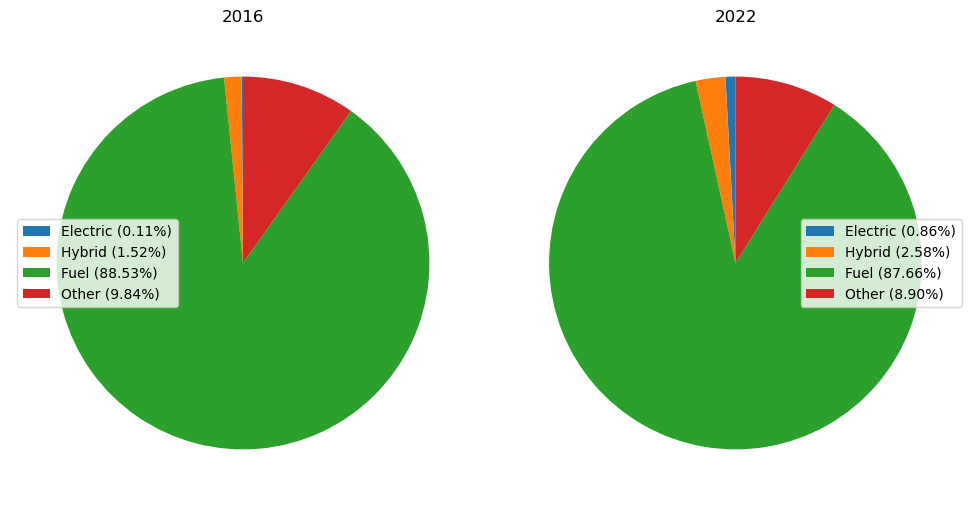
\includegraphics[scale=0.5]{img/output_1_0.png}
\end{center}

Um eine vergleichende Grafik zu erstellen, haben wir jeweils die Fahrzeugzahlen aus den Jahren 2016 und 2022 summiert. Die mit den Variablen erstellten Legenden (legend16 und legend22) enthalten prozentuale Anteile der einzelnen Fahrzeugtypen im Jahr 2016 bzw. 2022 im Verhältnis zur Gesamtanzahl der Fahrzeuge in diesen Jahren. Dem folgend haben wir zwei Kreisdiagramme für die jeweiligen Jahre erstellt. \\
Das Diagramm ermöglicht einen visuellen Vergleich der Veränderungen im Anteil verschiedener Fahrzeugtypen von 2016 zu 2022 und zeigt, dass sich die Zulassungen der Elektrofahrzeuge in diesem Zeitraum zwar um etwa das 8-fache erhöht haben, jedoch noch nicht 1\% der Gesamtzulassungen ausmachten.

\subsection{Anzahl Elektrofahrzeuge je Bundestaat}

\begin{minted}[bgcolor=LightGray,breaklines]{python}
# Anzahl Elektrofahrzeuge je Bundestaat
reg_per_state = registrations.groupby('State')['Electric'].sum()
reg_per_state = reg_per_state.reset_index(name='Count')
reg_per_state = pd.merge(reg_per_state, usa, on='State')

fig, axs = plt.subplots(1, 2, figsize=(10, 5))

axs[0].bar(reg_per_state['Abbreviation'], reg_per_state['Count'])
axs[0].set_title('Anzahl an registrierter E-Autos')
axs[0].set_xticks(axs[0].get_xticks())
axs[0].set_xticklabels(axs[0].get_xticklabels(), rotation=90, fontsize=8)

reg_pop = reg_per_state['Count'] / reg_per_state['Population']
axs[1].bar(reg_per_state['Abbreviation'], reg_pop)
axs[1].set_title('Anzahl an registrierter E-Autos / Einwohner')
axs[1].set_xticks(axs[1].get_xticks())
axs[1].set_xticklabels(axs[1].get_xticklabels(), rotation=90, fontsize=8)

plt.tight_layout()
plt.show()
\end{minted}

\begin{center}
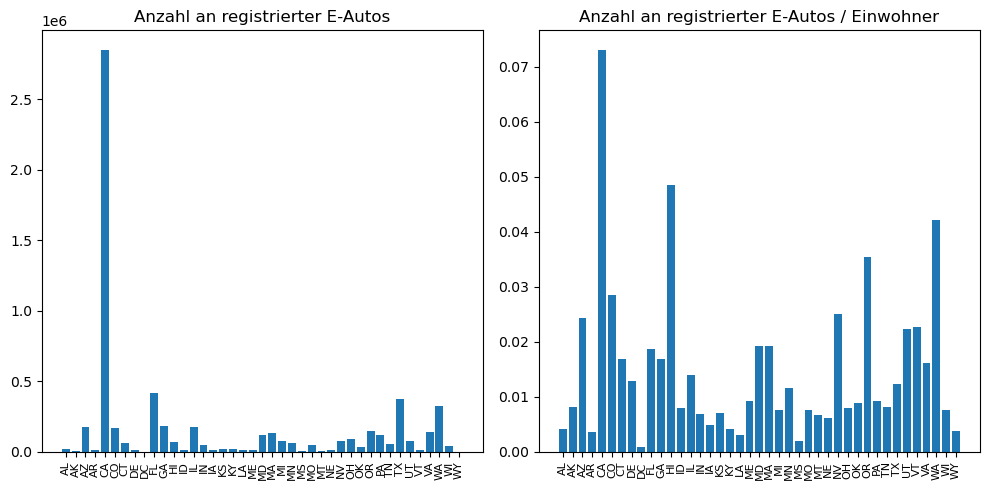
\includegraphics[scale=0.5]{img/output_2_0.png}
\end{center}

Um eine bessere Perspektive auf die Verteilung der E-Autos auf die Bundesstaaten zu bekommen, werden nun Zulassungen von Elektrofahrzeugen nach Bundesstaaten gruppiert, und die Summe der Elektrofahrzeuge pro Bundesstaat wird in einer neuen Spalte mit der Bezeichnung "Count" gespeichert. Mithilfe dieser Daten werden zwei Balkendiagramme erstellt. Das erste Diagramm zeigt die absolute Anzahl der registrierten Elektrofahrzeuge pro Bundesstaat (mit Abkürzung), während das zweite Diagramm die Anzahl der Elektrofahrzeuge pro Einwohner darstellt. 
Hier fällt stark auf, dass der Bundesstaat Kalifornien bei den absoluten Werten andere Bundesstaaten dominiert und auch bei der relativen Statistik weit vorne liegt. Doch holen hier vergleichsweise kleine Bundesstaaten wie Hawaii oder Washington stark auf. Hingegen sind die Staaten Florida und Texas, die nach absoluten Zahlen hohe Werte aufweisen beim relativen Vergleich eher das Schlusslicht. Kaum eine Präsenz in keiner von beiden Tabellen zeigen die Staaten Alabama, Arkansas, Iowa, Kentucky, Louisiana, Mississippi und Wyoming.

\subsection{Geografische Verteilung der Ladesäulen}

\begin{minted}[bgcolor=LightGray,breaklines]{python}
# Wie sind die Ladesäulen in den USA geografisch verteilt
map_center = [stations['Latitude'].mean(), stations['Longitude'].mean()]
my_map = folium.Map(location=map_center, zoom_start=5)
heat_data = [[row['Latitude'], row['Longitude']] for index, row in stations.iterrows()]
HeatMap(heat_data, radius=10, blur=7).add_to(my_map)
my_map
\end{minted}

\begin{center}
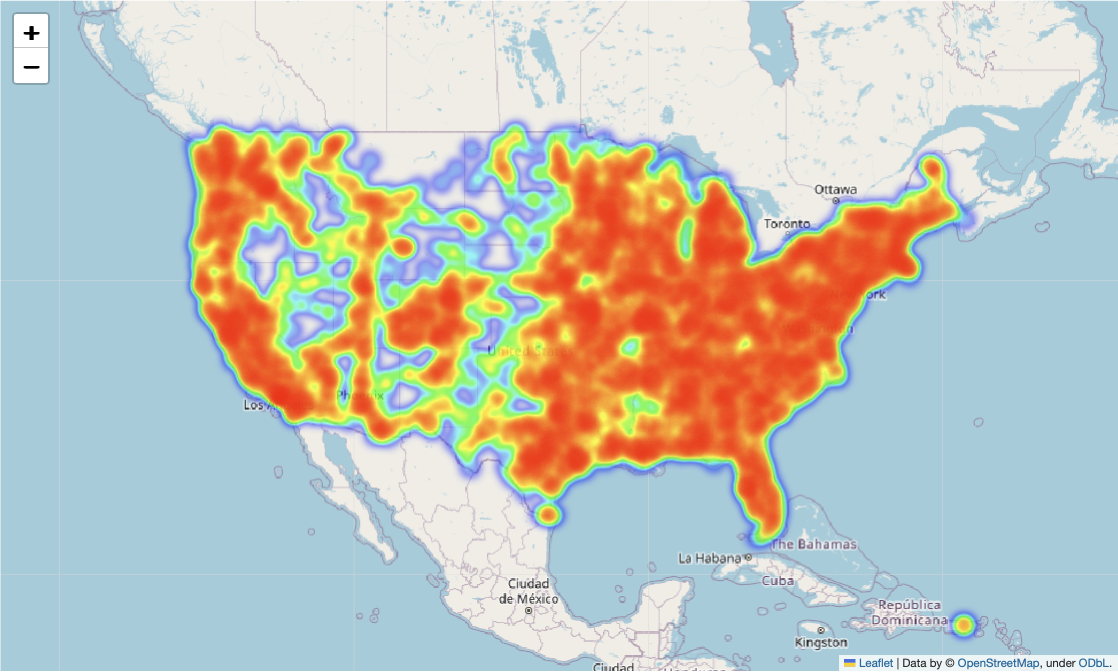
\includegraphics[scale=0.26]{img/output_3_0.png}
\end{center}

Die folgende Visualisierung zeigt die geografische Verteilung von Ladestationen in den USA. Zunächst wird der geografische Mittelpunkt der Ladestationen berechnet und als Zentrum für die Karte festgelegt. Mit folium.Map wird eine Karte erstellt. Danach werden die Breiten- und Längengrade der Ladestationen als Heatmap-Daten vorbereitet. Anschließend wird eine Heatmap mit diesen Koordinaten erstellt. Die Heatmap verdeutlicht, dass der gesamte Osten und Teile des Westens der USA eine gute Ladesäuleninfrastruktur haben, während besonders der Norden und die Mitte der USA große Lücken in ihrem Ladesäulennetz aufweisen.

\subsection{Anzahl der Ladesäulen je Bundestaat}

\begin{minted}[bgcolor=LightGray,breaklines]{python}
# Welche Bundestaaten haben die höchste bzw. niedrigste Anzahl an Ladesäulen
stations_per_state = stations.groupby('State').size().reset_index(name='Count')
stations_per_state = pd.merge(stations_per_state, usa, left_on='State', right_on='Abbreviation')

fig, axs = plt.subplots(1, 2, figsize=(12, 5))

axs[0].bar(stations_per_state['Abbreviation'], stations_per_state['Count'], color='green')
axs[0].set_title('Anzahl Ladesäulen')
axs[0].set_xticks(axs[0].get_xticks())
axs[0].set_xticklabels(axs[0].get_xticklabels(), rotation=90, fontsize=8)

stations_pop = stations_per_state['Count'] / stations_per_state['Population']
axs[1].bar(stations_per_state['Abbreviation'], stations_pop, color='green')
axs[1].set_title('Anzahl Ladesäulen / Einwohner')
axs[1].set_xticks(axs[1].get_xticks())
axs[1].set_xticklabels(axs[1].get_xticklabels(), rotation=90, fontsize=8)

plt.tight_layout()
plt.show()
\end{minted}

\begin{center}
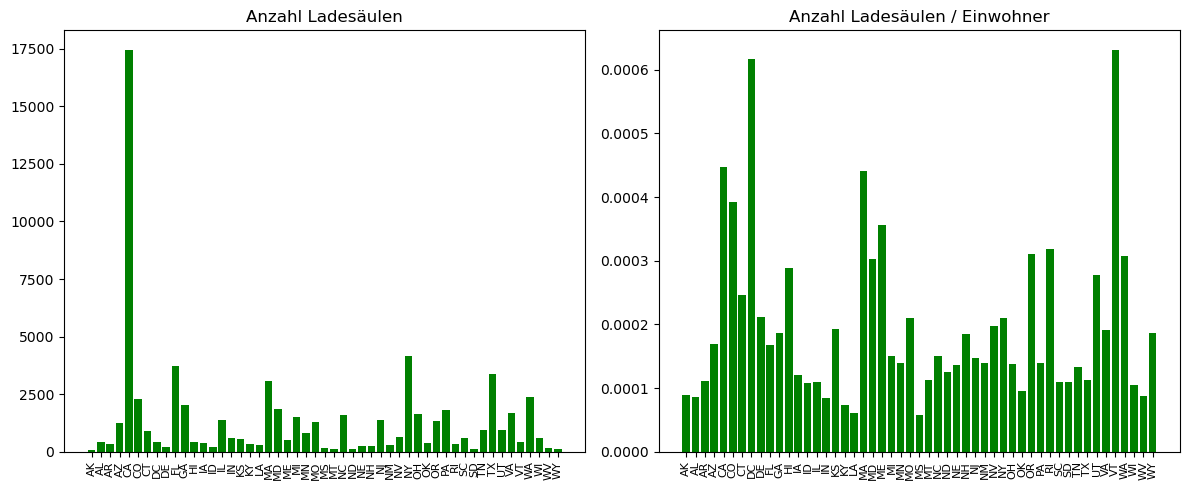
\includegraphics[scale=0.5]{img/output_4_0.png}
\end{center}

Zunächst werden die Ladestationen pro Bundesstaat gezählt, mit Bevölkerungsdaten verknüpft und in der Variable 'stations\_per\_state' gespeichert. Der erste Subplot zeigt die absolute Anzahl der Ladestationen (Y-Achse) pro Bundesstaat (X-Achse), während der zweite Subplot die Anzahl der Ladestationen je Einwohner (Y-Achse) pro Bundesstaat (X-Achse) darstellt. Besonders hervorstechend ist der Staat Kalifornien, welcher ein Vielfaches mehr an Ladesäulen hat, als der Staat mit den zweitmeisten Ladesäulen (New York), während Vermont, Washington, Massachusetts , District of Columbia (DC), als auch Colorado viele Ladesäulen pro Einwohner besitzen.

\subsection{Zeitliche Entwicklung der Anzahl der Ladesäulen + Trend}

\begin{minted}[bgcolor=LightGray,breaklines]{python}
# Wie hat sich die Anzahl der Ladesäulen im Laufe der Zeit entwickelt
# Gibt es einen Trend in der Eröffnung von Ladesäulen über die Jahre?
stations_trend = stations.groupby(stations['Open Date'].dt.year).size().reset_index(name='Count')
# es gibt eine Station 2024 im Datensatz
stations_trend = stations_trend[stations_trend['Open Date'] != 2024]

regressor = LinearRegression()
# Input-Variable
x_reg = stations_trend['Open Date']
# Output-Variable
y_reg = stations_trend['Count']

# Aufteilen in Test- und Trainingsdatensatz 
x_reg_train,x_reg_test,y_reg_train,y_reg_test=train_test_split(x_reg,y_reg,test_size=0.3, random_state= 1)

# Lernen des Modells
regressor.fit(np.array(x_reg_train).reshape(-1, 1), np.array(y_reg_train).reshape(-1, 1))

# Plot für Trainingsdaten
x_input = np.linspace(min(x_reg_train), 2030)
y_input = regressor.coef_ * x_input + regressor.intercept_
y_input = y_input.reshape(-1, 1)

# Trainingsfehler R^2 und MSE
y_reg_train_pred = regressor.predict(np.array(x_reg_train).reshape(-1,1))

fig, axs = plt.subplots(1, 2, figsize=(12, 4), gridspec_kw={'width_ratios': [4.5, 5.5]})

axs[0].set_title('Kumulative Anzahl der Ladesäulen über die Zeit')
axs[0].plot(stations_dev['Open Date'], stations_dev['Count'], linestyle='-')

axs[1].set_title('Entwicklung der Eröffnung von Ladesäulen pro Jahr')
axs[1].scatter(x = x_reg_train, y = y_reg_train, label='Eröffnungen')
axs[1].plot(x_input, y_input, c = 'r', label='Trendlinie')
axs[1].text(min(x_reg_train), max(y_reg_train), f'Coefficient: {regressor.coef_[0][0]:.3f}\nR^2: {r2_score(y_reg_train, y_reg_train_pred):.3f}\nMSE Train: {mean_squared_error(y_reg_train, y_reg_train_pred):.1f}', verticalalignment='top', bbox=dict(facecolor='white', alpha=0.3))
axs[1].legend(loc='lower right')

plt.tight_layout()
plt.show()
\end{minted}

\begin{center}
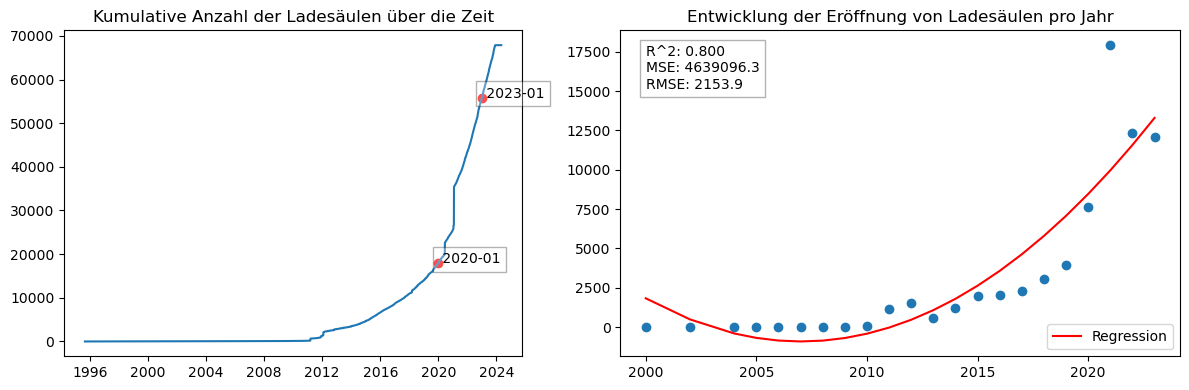
\includegraphics[scale=0.5]{img/output_5_0.png}
\end{center}

Lorem ipsum dolor sit amet, consetetur sadipscing elitr, sed diam nonumy eirmod tempor invidunt ut labore et dolore magna aliquyam erat, sed diam voluptua. At vero eos et accusam et justo duo dolores et ea rebum. Stet clita kasd gubergren, no sea takimata sanctus est Lorem ipsum dolor sit amet. Lorem ipsum dolor sit amet, consetetur sadipscing elitr, sed diam nonumy eirmod tempor invidunt ut labore et dolore magna aliquyam erat, sed diam voluptua. At vero eos et accusam et justo duo dolores et ea rebum. Stet clita kasd gubergren, no sea takimata sanctus est Lorem ipsum dolor sit amet. Lorem ipsum dolor sit amet, consetetur sadipscing elitr, sed diam nonumy eirmod tempor invidunt ut labore et dolore magna aliquyam erat, sed diam voluptua. At vero eos et accusam et justo duo dolores et ea rebum. Stet clita kasd gubergren, no sea takimata sanctus est Lorem ipsum dolor sit amet.   
Duis autem vel eum iriure dolor in hendrerit in vulputate velit esse molestie consequat, vel illum dolore eu feugiat nulla facilisis at vero eros et accumsan et iusto odio dignissim qui blandit praesent luptatum zzril delenit augue duis dolore te feugait nulla facilisi. Lorem ipsum dolor sit amet,

\subsection{Ladeinfrastruktur im Vergleich zur Anzahl registrierter E-Autos}

\begin{minted}[bgcolor=LightGray,breaklines]{python}
# Korrelationen Infrastrukturentwicklung
stations_data = stations.groupby(stations['Open Date'].dt.year).size().cumsum().reset_index(name='Count')
stations_data = stations_data.rename(columns={'Open Date': 'Year'})

registrations_data = registrations.groupby(registrations['Year'])['Electric'].sum().reset_index(name='Count')

merge = pd.merge(stations_data, registrations_data, on='Year')

# Korrelationskoeffizient berechnen
correlation_coefficient = merge['Count_x'].corr(merge['Count_y'])

plt.figure(figsize=(10,4))

# Ladesäulen
sns.lineplot(x='Year', y='Count', data=stations_data, label='Ladesäulen', marker='o')

# Elektrofahrzeuge
sns.lineplot(x='Year', y='Count', data=registrations_data, label='Elektrofahrzeuge', marker='o')

plt.title(f'Entwicklung der Ladeinfrastruktur im Vergleich zu Elektrofahrzeugen\nKorrelationskoeffizient: {correlation_coefficient:.3f}')
plt.xlabel('Jahr')
plt.ylabel('Anzahl')
plt.legend()
plt.show()
\end{minted}

\begin{center}
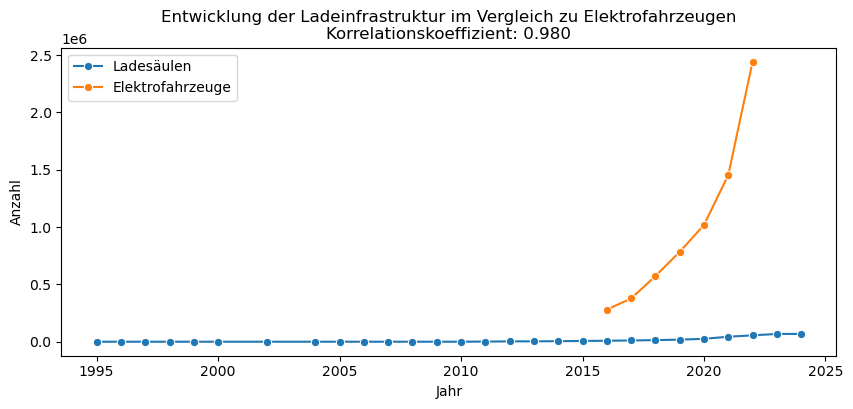
\includegraphics[scale=0.5]{img/output_6_0.png}
\end{center}

Lorem ipsum dolor sit amet, consetetur sadipscing elitr, sed diam nonumy eirmod tempor invidunt ut labore et dolore magna aliquyam erat, sed diam voluptua. At vero eos et accusam et justo duo dolores et ea rebum. Stet clita kasd gubergren, no sea takimata sanctus est Lorem ipsum dolor sit amet. Lorem ipsum dolor sit amet, consetetur sadipscing elitr, sed diam nonumy eirmod tempor invidunt ut labore et dolore magna aliquyam erat, sed diam voluptua. At vero eos et accusam et justo duo dolores et ea rebum. Stet clita kasd gubergren, no sea takimata sanctus est Lorem ipsum dolor sit amet.

\subsection{Korrelation zw. Anzahl der Ladesäulen und anderen Faktoren}

\begin{minted}[bgcolor=LightGray,breaklines]{python}
# Korrelation zw. der Anzahl Ladesäulen und anderen Faktoren, wie der Bevölkerung, Bevölkerungsdichte?
stations_corr = stations.groupby(stations['State']).size().reset_index(name='Count')
stations_corr = pd.merge(stations_corr, usa, left_on='State', right_on='Abbreviation')
stations_corr['Population density'] = stations_corr['Population'] / stations_corr['Land_area']

# Korrelationsmatrix erstellen
correlation_matrix = stations_corr[['Count', 'Population', 'Population density']].corr()

# Heatmap der Korrelationsmatrix erstellen
plt.figure(figsize=(9, 3))
sns.heatmap(correlation_matrix, annot=True, cmap='coolwarm', fmt='.2f', linewidths=.5)
plt.title('Korrelationsmatrix zw. Anzahl Ladesäulen und Bevölkerung / Bevölkerungsdichte')
plt.yticks(rotation=0)
plt.show()
\end{minted}

\begin{center}
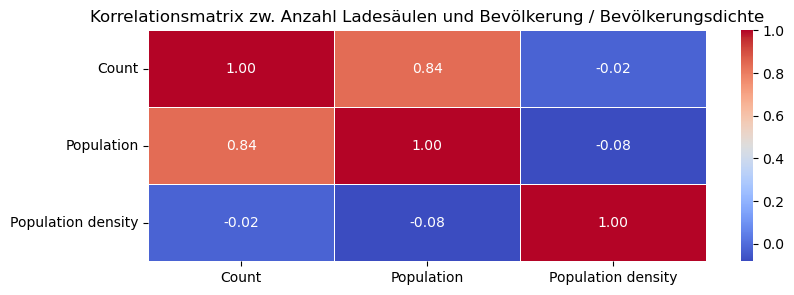
\includegraphics[scale=0.5]{img/output_7_0.png}
\end{center}

Im Vorliegenden haben wir die Korrelation zwischen Anzahl der Ladesäulen, Bevölkerung und Bevölkerungsdichte in den USA analysiert. Zunächst werden die Ladestationen pro Bundesstaat gezählt und mit Bevölkerungsdaten verknüpft, daraufhin wird die Bevölkerungsdichte berechnet und gespeichert. Eine Korrelationsmatrix zeigt die Beziehung zwischen Ladestationen, Bevölkerung und Dichte. Die Heatmap visualisiert die Korrelationen und ermöglicht eine einfache Interpretation der Verbindungen zwischen Ladesäulen und Bevölkerungsfaktoren. 
So zeigt die Heatmap, dass die Korrelation zwischen Anzahl der Ladesäulen und Bevölkerungsanzahl besonders hoch ist, die Ladesäulenanzahl jedoch nur eine geringe Korrelation zur Bevölkerungsdichte hat. Allgemein lässt sich sagen, dass eine hohe Bevölkerungszahl mit vielen Ladesäulen einhergeht.

\subsection{Korrelation zw. Anzahl der E-Autos und politischer Einstellung}

\begin{minted}[bgcolor=LightGray,breaklines]{python}
# registrations / plolitischer Mehrheit - stations / politischer Mehrheit 
reg_vote = registrations[registrations['Year'] == 2022]
reg_vote = pd.merge(registrations, usa, on='State')
reg_vote = reg_vote.groupby('Vote')['Electric'].sum().reset_index(name='Count')

stations_vote = pd.merge(stations, usa, left_on='State', right_on='Abbreviation')
stations_vote = stations_vote.groupby('Vote').size().reset_index(name='Count')

fig, axs = plt.subplots(1, 2, figsize=(10, 5))

axs[0].pie(reg_vote['Count'], autopct='%1.1f%%', startangle=90, colors=['blue', 'lightblue', 'lightcoral', 'red', 'grey'])
axs[0].set_title('Registrierte E-Autos (2022) nach politischer Mehrheit')
axs[0].set_xticks(axs[0].get_xticks())
axs[0].set_xticklabels(axs[0].get_xticklabels(), rotation=90, fontsize=8)
axs[0].legend(stations_vote['Vote'], loc="upper left")

axs[1].pie(stations_vote['Count'], autopct='%1.1f%%', startangle=90, colors=['blue', 'lightblue', 'lightcoral', 'red', 'grey'])
axs[1].set_title('Anzahl Ladesäulen nach politischer Mehrheit')
axs[1].set_xticks(axs[1].get_xticks())
axs[1].set_xticklabels(axs[1].get_xticklabels(), rotation=90, fontsize=8)
axs[1].legend(stations_vote['Vote'], loc="upper right")

plt.tight_layout()
plt.show()
\end{minted}

\begin{center}
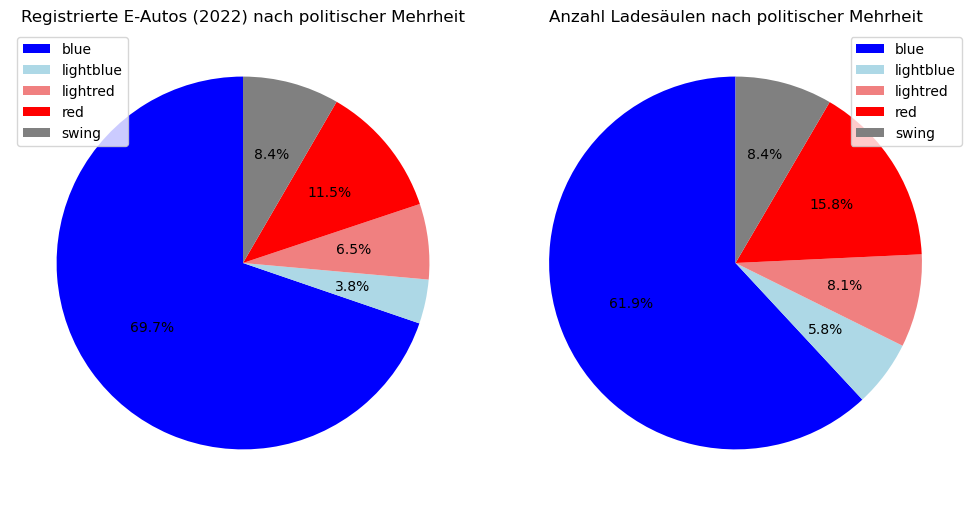
\includegraphics[scale=0.5]{img/output_8_0.png}
\end{center}

Nun möchten wir analysieren, wie die politischen Ausrichtung der Bundesstaaten mit Registrierungen von E-Autos zusammenhängt. Dazu nutzen wir die Registrierungsdaten pro Bundesstaat aus 2022 und vereinigen ihn mit den politischen Ausrichtungen des jeweiligen Staates aus einem anderen Datensatz. Analog geschieht das ebenfalls mit der Anzahl von Ladesäulen pro Bundesstaat.
Daraufhin visualisieren wir mit zwei Kreisdiagrammen ein klares Bild: Die E-Mobilität ist in den 'blue states' bzw. 'light blue states'  also in Bundesstaaten, in denen vier bzw. drei der letzten US-Wahlen von den Demokraten gewonnen wurden, weitaus entwickelter und beliebter. Der Grund dafür könnte die konservative Grundstimmung der 'red states' bzw. 'light red states' sein. In jenen Staaten wurde vier bzw. drei von vier Legislaturperioden republikanisch gewählt, daher ist die Abneigung gegenüber E-Mobilität höher. In den 'swing states' (zwei von vier Legislaturperioden republikanisch bzw. demokratisch gewählt) gibt es keine große Auffälligkeit.



